\documentclass[a3,convert]{standalone}
\usepackage{pgfplots}
\usepgfplotslibrary{smithchart}    
\usepgfplotslibrary{polar}   
\usepackage{siunitx} 
\usepackage{tikz}
\pgfplotsset{compat=1.18}
\usetikzlibrary{calc,intersections,through}
\usepackage{comment}

\begin{document}
    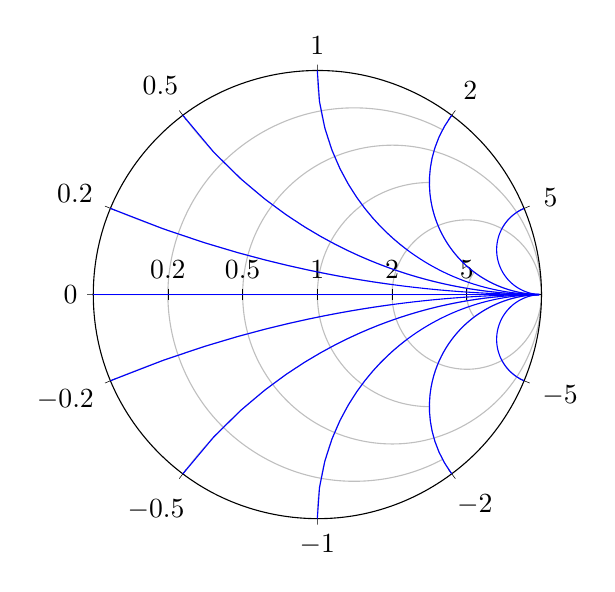
\begin{tikzpicture}
    \begin{smithchart}
      % Reactance plot
      \addplot[domain=0:90,samples=600,color=blue]{.5};
      \addplot[domain=0:90,samples=600,color=blue]{1};
      \addplot[domain=0:90,samples=600,color=blue]{2};
      \addplot[domain=0:90,samples=600,color=blue]{.2};
      \addplot[domain=0:90,samples=600,color=blue]{5};
      \addplot[domain=0:90,samples=600,color=blue]{0};
      \addplot[domain=0:90,samples=600,color=blue]{-.5};
      \addplot[domain=0:90,samples=600,color=blue]{-1};
      \addplot[domain=0:90,samples=600,color=blue]{-2};
      \addplot[domain=0:90,samples=600,color=blue]{-.2};
      \addplot[domain=0:90,samples=600,color=blue]{-5};


      % Resistance plot - orange
      

      %\addplot+[mark=*,only marks,samples at={.5,.51,...,5},
      %  mark options={solid},color={orange},mark size=.2,line width=1](.5,x);
      % Resistance plot - red
      %\addplot+[mark=*,only marks,samples at={0,.01,...,.5},
      %  mark options={solid},color={red},mark size=.2,line width=1](1,x);

      
    \end{smithchart}
  \end{tikzpicture}
\end{document}
